\section{Outliers}
\subsection{Finding Baseline}
In this outlier analysis section, our primary objective was to identify the top outliers in the dataset using three well-established methods- 
\texttt{Local Outlier Factor, Isolation Forest}, and \texttt{Angle-Based Outlier Detection}. 
To establish a baseline for model performance, we initially employed two supervised learning algorithms- 
\texttt{Decision Tree} and \texttt{K-Nearest Neighbors}.
To enhance the alignment between the later module tasks we defined a categorical target variable, \texttt{rating\_bin}, 
by dividing the continuous \texttt{averageRating} into six distinct classes. 
The classes were defined as follows:
\begin{center}
    0 = [0-5); 1 = [5-6); 2 = [6-7); 3 = [7-8); 4 = [8-9); and 5 = [9-10]\\
\end{center}
The value count for each class was 12856, 19576, 37032, 49164, 25414, and 5489 respectively.\\
We then performed a grid search with cross-validation \texttt{(GridSearchCV)} on both models to identify the best hyperparameters. 
Since our dataset was large, we conducted the grid search on a 10\% stratified sample to optimize computational efficiency. 
For K-NN, the optimal parameters were- 
\begin{center}
    metric = 'manhattan', n\_neighbors = 122, weights = 'distance'
\end{center} 
However, to strike a balance between accuracy and computational efficiency, we restricted our model to use \texttt{50 n\_neighbors}. 
For Decision Tree, the optimal parameters were-
\begin{center}
    criterion = 'gini', max\_depth = 10, min\_samples\_leaf = 4, min\_samples\_split = 10, splitter = 'random'
\end{center}
We trained both models on the entire training dataset and evaluated their performance on the test set. 
We split our training dataset into training (80\%) and validation (20\%) sets. We computed the baseline accuracy 
without removing any outliers, which was \texttt{36\% for K-NN} and \texttt{32\% for Decision Tree}.

\subsection{Finding Threshold}
Next, we applied the three outlier detection methods to identify and remove outliers from the training dataset.
We experimented with different contamination levels \texttt{(0.01, 0.05, 0.1)} to 
determine the optimal proportion of outliers to remove.
After removing the identified outliers, we retrained both models on the cleaned training dataset and evaluated their performance on the test set.
We observed that removing outliers generally improved model accuracy, but different contamination levels had no significant impact on the results as shown in table \ref{tab: threshold}.
Only the results from LOF with a contamination level of 0.1 showed an improvement of 1\%. 
Therefore, we fixed the contamination level at 10\% for all three methods to maintain consistency. 
Subsequently, we combined the results of the three methods by aggregating the outlier score and 
removed those rows that were flagged as outliers by at least \texttt{two out of the three methods}, 
which accounted for approximately \texttt{3\%} of the dataset.


\begin{table}[]
\centering
\begin{tabular}{|l|l|l|l|l|}
\hline
 &  & \textbf{LOF} & \textbf{IF} & \textbf{ABOD} \\ \hline
\multirow{2}{*}{\textbf{1\%}} & \textbf{KNN} & 42 & 42 & 41 \\ \cline{2-5} 
 & \textbf{DT} & 39 & 39 & 40 \\ \hline
\multirow{2}{*}{\textbf{5\%}} & \textbf{KNN} & 42 & 42 & 41 \\ \cline{2-5} 
 & \textbf{DT} & 39 & 39 & 40 \\ \hline
\multirow{2}{*}{\textbf{10\%}} & \textbf{KNN} & \textbf{43} & 42 & 41 \\ \cline{2-5} 
 & \textbf{DT} & \textbf{40} & 39 & 40 \\ \hline
\end{tabular}
\caption{Accuracy at different threshold}
\label{tab: threshold}
\end{table}

\subsection{Outlier Detection Conclusion}
In conclusion, our anomaly detection task revealed a consistent trend: both models \texttt{KNN} and \texttt{DT} performed better than the 
baseline after the removal of outliers. This outcome sets the foundation for our subsequent focus on model 
explainability in the later sections.\\ 
From the T-SNE visualization, we observed that \texttt{LOF} predominantly 
identified outliers at the edges of the data distribution \ref{fig:LOF}, whereas \texttt{IF} detected 
them primarily within a clustered region \ref{fig:ISF}. \texttt{ABOD}, on the other hand, captured outliers both at 
the edges and within dense clusters \ref{fig:ABOD}. This variation can be explained by the fundamental 
differences between the algorithms: \texttt{LOF} emphasizes anomalies in low-density regions, 
while \texttt{IF} isolates points distant from the main distribution. 
\texttt{ABOD}, which evaluates outliers based on the angular relationships of points, reflects a hybrid behavior by 
marking anomalies in both sparse and dense regions. Importantly, since the dataset is dominated by a 
single high-density region, most points lack anomalous neighbors, explaining why \texttt{ABOD} highlighted relatively 
fewer strong anomalies. To ensure computational efficiency, we implemented the 'fast' version of \texttt{ABOD}, 
which approximates angle-based detection using a specified number of neighbors rather than exhaustively 
computing angles across all data points. \\
Overall, as we can see from table \ref{tab: threshold} the removal of outliers with different threshold led to only marginal gains in predictive performance.
However, the differences in detection patterns across methods provide valuable insights into the structure and density 
of the data distribution, reinforcing the importance of combining multiple approaches for a more 
comprehensive anomaly detection strategy. Therefore, we combined the results of all three methods to identify the common outliers.





\begin{figure}[htbp]
    \centering
    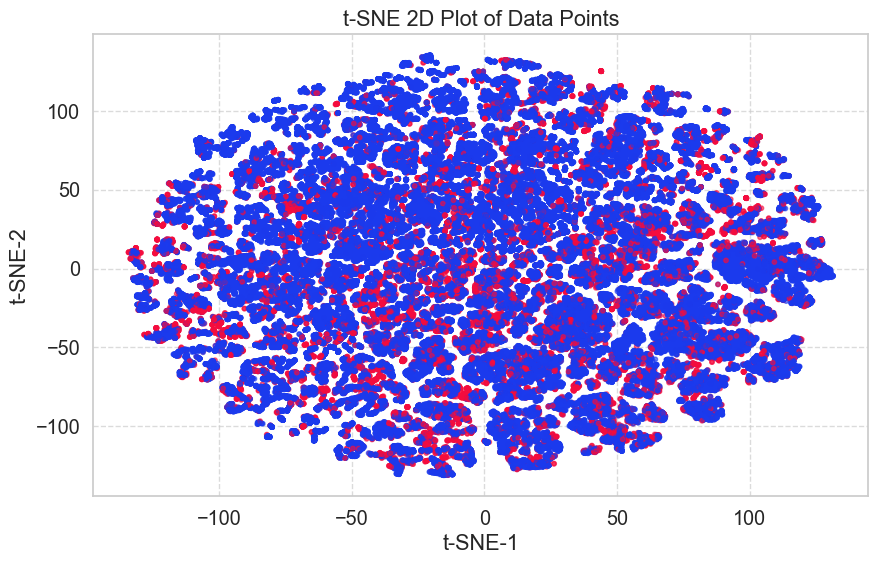
\includegraphics[width=0.7\textwidth]{plotsss/LOF.png} % path to your image
    \caption{T-SNE visualization showing LOF outlier detection patterns.}
    \label{fig:LOF}
\end{figure}
\begin{figure}[htbp]
    \centering
    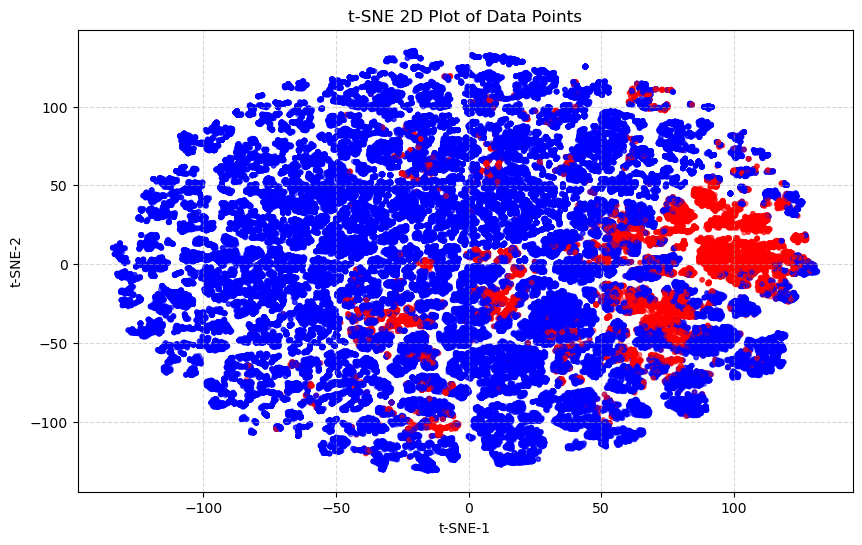
\includegraphics[width=0.7\textwidth]{plotsss/ISF.png} % path to your image
    \caption{T-SNE visualization showing IF outlier detection patterns.}
    \label{fig:ISF}
\end{figure}
\begin{figure}[htbp]
    \centering
    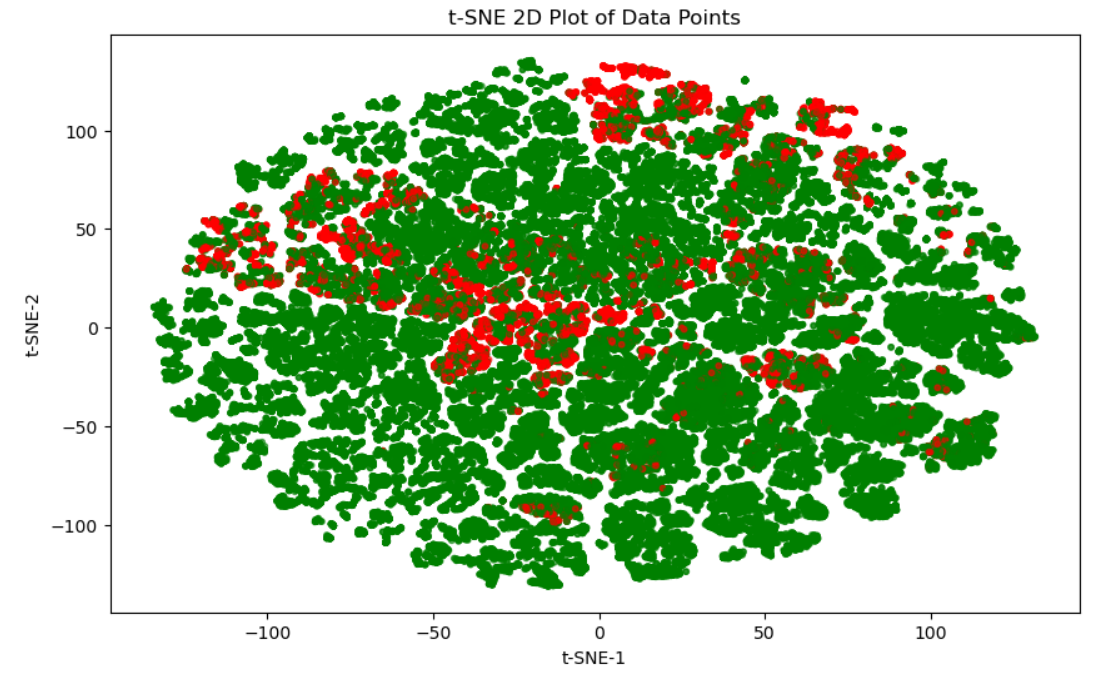
\includegraphics[width=0.7\textwidth]{plotsss/ABOD.png} % path to your image
    \caption{T-SNE visualization showing ABOD outlier detection patterns.}
    \label{fig:ABOD}
\end{figure}
